\documentclass[12pt]{article}
\usepackage{amsmath}
\usepackage{amsfonts}
\usepackage[utf8]{inputenc}
\usepackage{cite}
\usepackage{geometry}
\usepackage{graphicx} % Required for including images
\usepackage{setspace}  % For line spacing
\usepackage{parskip}   % For extra space between paragraphs
\usepackage{hyperref}  % For clickable links
\usepackage{float}  % For figure placement.
\geometry{margin=1in}

% Set line spacing to 1.5
\onehalfspacing

\title{Are Social Networks Naturally Hierarchical?}
\date{June 1, 2025}
\author{Brian Kay}

\begin{document}

\maketitle

\section{Summary}
After a reading group session on \textit{Neither Vertical Nor Horizontal} by Rodrigo Nunes, our group had a discussion about
whether hierarchy was "natural" and what hierarchy is. I wanted to study if it was true that hierarchies naturally
formed in social networks. To do this, I wrote a program to randomly generate vertex-edge graphs and test for the
appearance of hierarchy. In this simple experiment, a model of a growing social network does
tend toward hierarchy. We don't have to take this fatalistically. It may show that if we value equality, it takes
conscious effort and planning to distribute influence and counteract the inequalities in hierarchy.

\section{Methods}

\subsection{Modeling Social Networks}

There are several types of graphs used as
models of social networks. I used one of the oldest, \textbf{Price's Model}~\cite{wikipediaPricesModel},
which was intended to understand the growth of
the number of academic citations of published papers. The idea of the model is that existing papers will be cited by new
papers in proportion to how much they've already been cited. This is called \textit{preferential attachment}.
The growth of citations in the model is similar to the
actual distribution of paper citations. To apply this model to the growth of a volunteer organization, imagine
that the relationships are influence instead of citations.
Person $A$ influences person $B$, $A \rightarrow B$, and that if a new person $C$ enters an organization, they'll be influenced by
people who are already influential, so the social graph will grow by preferential attachment.

Formally, such a network is a mathematical graph~\cite{wikipediaGraphTheory} of vertices (nodes) and edges, $G=(V,E)$ where the edges have a direction.
In Price's Model, the probability of a new edge connecting to any node with a degree $k$ is $\frac{(k + 1) p_k}{m + 1}$,
where $p_k$ is the fraction of nodes with degree $k$ and $m$ is the mean number of
attachments.

\subsection{What is Hierarchy?}

To test for hierarchy, I use a measure called \textbf{graph agony}~\cite{tatti2014faster}. In a hierarchical ranking of nodes, the graph agony
is the weighted count of the edges that have a direction that is counter to the
hierarchy. So, a ranking assignment that is consistent with hierarchy should have a low graph agony.

Given a directed graph $G=(V,E)$ and a
ranking function $r:V \rightarrow \mathbb{Z}$ assigning integer ranks to nodes,
the agony of an edge $(u,v)$ is defined as:
$agony(u,v)=max(0,r(u) - r(v)+1)$. and

$Total Agony(G,r)= \sum_{(u,v) \in E} max(0,r(u) - r(v)+1)$.

\textbf{Hierarchies} can be found in graphs by finding the ranking of nodes that minimizes graph agony:

$\min_{r : V \to \mathbb{Z}} \sum_{(u,v) \in E} max(0,r(u) - r(v)+1)$

\subsection{Experiment}

Minimizing graph agony is computationally complex. There are optimized methods for it, but I only wanted small
networks that I could visualize, so I used a brute-force method of randomly selecting rankings and keeping the one
that created the lowest graph agony. I ran 12 trials of 12 node graphs, starting with 2 nodes and a mean attachment of
2, and picked some representative results. Graphs are shown with nodes arranged in a circle
rather than trying to arrange them for the hierarchy.

The brute-force search finds hierarchies in these small graphs,
with only a few edges being directed against the ranking
hierarchy. Often, graphs have two top-level nodes (rank 0), the first two in the graph ($A$ and $B$), as shown
in Figure~\ref{fig:multiple-highest-nodes}.
\begin{figure}[H]
    \centering
    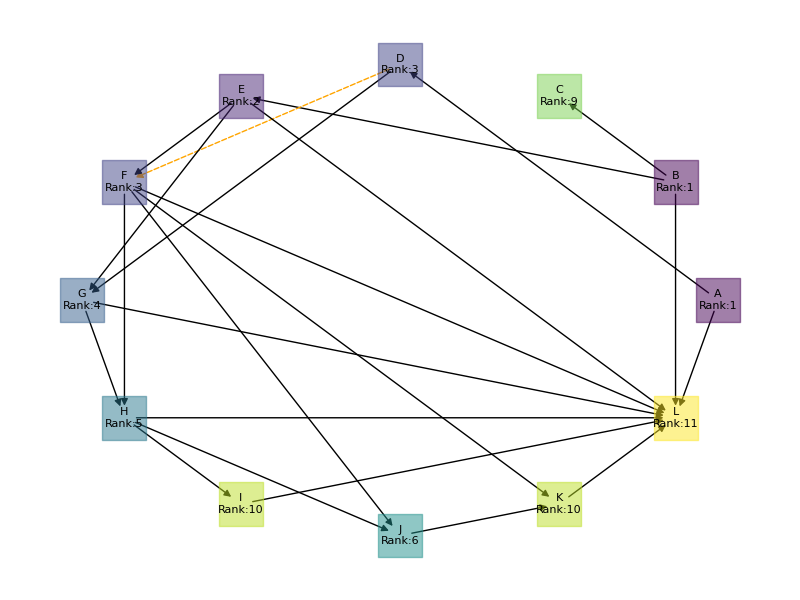
\includegraphics[width=0.8\textwidth]{images/2025-06-01-15:51:09.145097-network.png}
    \caption{Two Highest Nodes (Rank 1)}
    \label{fig:multiple-highest-nodes}
\end{figure}

More rarely, graphs have one top node, as shown in Figure~\ref{fig:one-top-node}.
\begin{figure}[H]
    \centering
    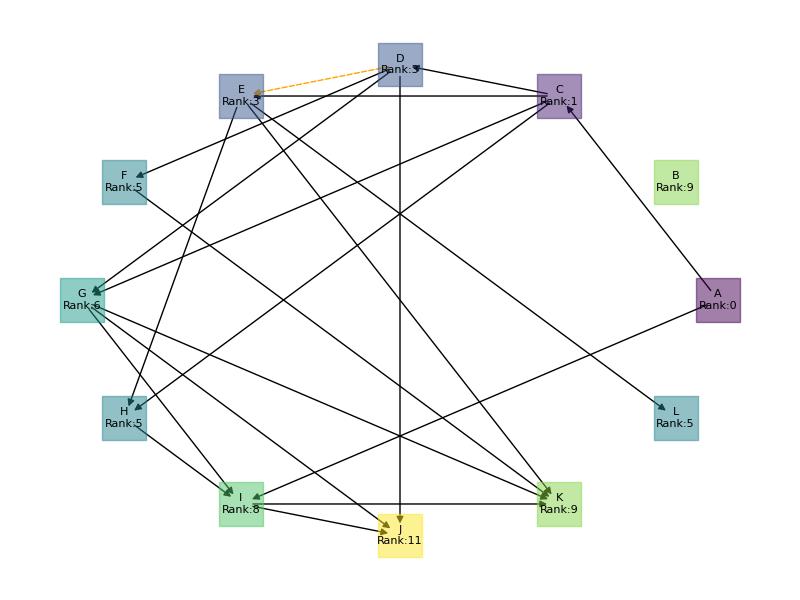
\includegraphics[width=0.8\textwidth]{images/2025-06-01-15:51:36.967731-network.png}
    \caption{One Top-Most Node (Rank 0)}
    \label{fig:one-top-node}
\end{figure}

Both graphs shown have one edge that is directed against the hierarchy, shown as an orange dotted line.

\section{Conclusions}

Under the simple assumptions of Price's Model, growing social networks tend to organize in hierarchies. Humans are
adaptable and creative, and we can't make a survey of all social arrangement throughout human existence,
so we shouldn't make many conclusions about the essential features of social networks, but given the ubiquity of
hierarchies in contemporary organizations, it is reasonable to conclude that under many conditions, people tend to
organize in hierarchies. This shouldn't mean that we are fated to act under hierarchies. If
members of an organization value equality, they must counter tendencies to hierarchy through education, training,
and formal organizing techniques such as term limits and distributed leadership.

\bibliographystyle{plain}      % Choose style: plain, IEEEtran, etc.
\bibliography{references}      % This links to references.bib

\end{document}

